\documentclass{IEEEtran}
\usepackage{graphicx, float}
\usepackage{soul}
\usepackage{listings}

\usepackage[hidelinks]{hyperref}
\usepackage[backend=biber]{biblatex}
\addbibresource{references.bib}

 %\renewcommand{\bottomfraction}{.7}
 %\renewcommand{\textfraction}{.15}
 %\renewcommand{\floatpagefraction}{.66}
 %\renewcommand{\dbltopfraction}{.66}
 %\renewcommand{\dblfloatpagefraction}{.66}
 %\setcounter{topnumber}{9}
 %\setcounter{bottomnumber}{9}
 %\setcounter{totalnumber}{20}
 %\setcounter{dbltopnumber}{9}

 
\newcommand{\makeBasicPlottingFig}{%
\begin{figure*}[tbh]
 \centering
% \includegraphics[width=\linewidth]{basicPlotting}
 \includegraphics[width=1.0\textwidth]{figures/basicPlotting.pdf}
 \caption{A selection of basic plots from PyQtGraph's suite of examples.}
 \label{fig:basicPlotting}
\end{figure*}}

\newcommand{\makePtreeExFig}{%
\begin{figure}[!htbp]
\centering
\includegraphics[width=\columnwidth]{figures/pg_ptree_ex.png}
\caption{Sample use of parameter trees for user interaction, where various image processing parameters can be quickly updated. The displayed image reflects these changes in real-time.}
 \label{fig:ptreeEx}
\end{figure}}

\newcommand{\makeNeuralNetFig}{%
\begin{figure*}
\centering
\includegraphics[width=0.8\textwidth]{figures/neuralNetFig.png}
\caption{Application demonstrating how parameter trees, real-time plotting updates, signal hooks, and more can facilitate rapid prototyping and impacts of architectural changes.}
 \label{fig:neuralNetFig}
\end{figure*}}

\newcommand{\makeLineBenchmarkFig}{%
\begin{figure}[!b]
\centering
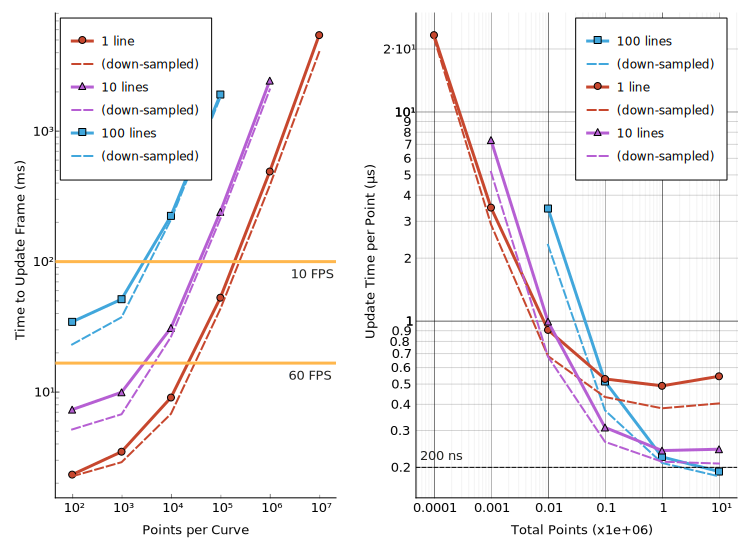
\includegraphics[width=\columnwidth]{figures/lineBenchmark.pdf}
\caption{Line speed benchmark. The time to render 1, 10 or 100 lines of data is shown for varying numbers of points per line. All data was created using an AMD 5900x Ryzen 9 CPU. Left: Time per update over points per curve. The thresholds for achieving 10 and 60 frames/s are shown by horizontal lines. Right: Update time per point, plotted over the total number of points. For more than 100,000 points, the line-plotting time becomes dominant, and the results converge to 200\,ns per point for both 10 and 100 curves, while plotting all points as a single curve increases the time to 500--600\,ns per point.}
 \label{fig:lineSpeed}
\end{figure}
}
 %13-inch 
 
\newcommand{\makeMatplotlibComparison}{%
\begin{figure}[bth]
\centering
\includegraphics[width=0.9\columnwidth]{figures/pg-mpl-comparison_no_interpolation.png}
\caption{Performance test with PyQtGraph and Matplotlib widgets embedded in a Qt5 application. Over a wide range of image sizes, PyQtGraph completes drawing approximately 75--150 times faster, taking only 5.4\,ms in this example of a 4000\texttimes4000 image. The test is performed without GPU acceleration in a Microsoft Windows environment, and both libraries are set to sub-sample without interpolation. Free-to-use test images are provided by the \href{https://unsplash.com/}{``Unsplash''} service.} 
\label{fig:mpl}
\end{figure}
}

 \newcommand{\makeARBBenchmarkFig}{
 \begin{figure}[tbh]
 \centering
 \includegraphics[width=\columnwidth]{figures/makeARGBBenchmark.pdf}
 \caption{Image speed benchmark. The time to update an image frame is shown for different data formats. Left: Using optimized NumPy processing (purple lines), the drawing time is log-scale linear with the number of pixels over a wide range. GPU accelerated CUDA processing using CuPy (green lines) describe a more complex relationship with image size. The need to copy data to and from the GPU creates additional overhead, but as image size grows, the faster processing speed becomes sufficient to compensate for that overhead. The choice of various extra processing tasks like LUTs (dashed lines) show the same basic trends. Alternatively, PyQtGraph's image rendering pipeline can be accelerated in Numba is available on the system.  Benchmarks with Numba (blue lines) can be seen as have performance between that of CuPy and NumPy only. Right: For input data in uint16 format, CUDA processing is particularly advantageous and can provide an almost four-fold reduction in drawing time. Benchmarks were performed on an AMD 5900x Ryzen 9 CPU and an NVIDIA RTX 3080 discrete GPU.}
 \label{fig:makeARGB}
 \end{figure}
 }
 
\newcommand{\makeMonitoringFig}{%
\begin{figure}[!htbp]
\centering
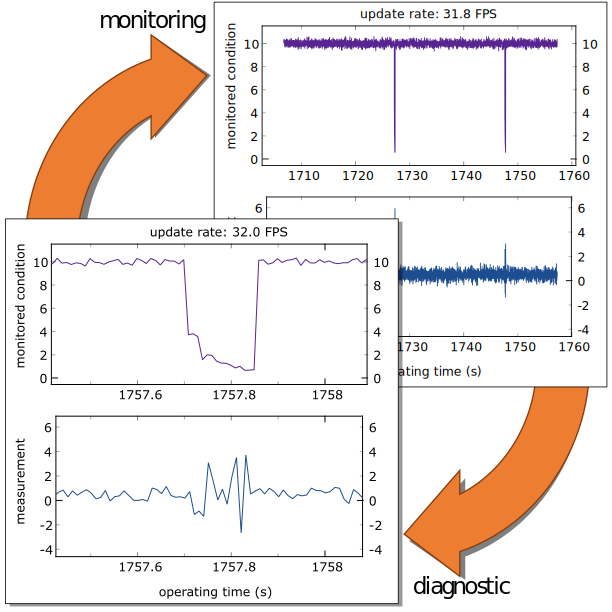
\includegraphics[width=\columnwidth]{figures/monitoring_example_vector.pdf}
\caption{Monitoring and diagnostic of a (simulated) experiment with intermittent failures. Incoming data at 100 samples/s for two measurement channels is recorded into a rolling 5,000 point buffer and continuously displayed at 30 frames/s. When a failure is observed, it can quickly be brought into focus with simple mouse interactions (click-and-drag and mousewheel zoom) for inspection, or to record accurate time stamps. Afterwards, a single click returns the view to automatic scaling without loss of any incoming data.}
 \label{fig:monitoring}
\end{figure}
}



%% Paper title.
\title{Semi-Supervised Semantic Annotator (S3A): Toward Efficient Semantic Image Labeling}

%% This is how authors are specified in the journal style

%% indicate IEEE Member or Student Member in form indicated below
\author{Nathan Jessurun, Daniel E. Capecci, Olivia P. Dizon-Paradis, Damon L. Woodard, Navid Asadizanjani}
\begin{document}

\maketitle

\begin{abstract}
Most semantic image annotation platforms suffer severe bottlenecks when handling large images, complex regions of interest, or numerous distinct foreground regions in a single image. We have developed the Semi-Supervised Semantic Annotator (S3A) to address each of these issues and facilitate rapid collection of ground truth pixel-level labeled data. Such a feat is accomplished through a robust and easy-to-extend integration of arbitrary python image processing functions into the semantic labeling process. Importantly, the framework devised for this application allows easy visualization and machine learning prediction of arbitrary formats and amounts of per-component metadata. To our knowledge, the ease and flexibility offered are unique to S3A among all open-source alternatives. S3A is available through pypi.org (\url{https://pypi.org/project/s3a/}) and GitLab (\url{https://gitlab.com/s3a/s3a}).
\end{abstract}

\section{Introduction}
Labeled image data is essential for tuning and evaluating the performance of machine learning applications.
Such labels are typically defined with approximate enclosing shapes (i.e. simple polygons or parametric shapes), which tend to misrepresent more complex components.
% While this streamlines the labeling process, it misrepresents more complex components.
When high accuracy is required, labels must be specified at or close to the pixel-level – a process known as semantic labeling or semantic segmentation.
A detailed description of this process is given in \cite{chengSurveyAnalysisAutomatic2018}. Examples can readily be found in several popular datasets such as COCO, depicted in \autoref{fig:sampleSegData}.

\makeSampleSegFig

% However, a wide variety of applications require pixel-level accuracy, ranging from hardware assurance to medical imaging.
% Alternatively, semantic segmentation is a technique providing pixel-level accuracy which avoids poor foreground representation~\cite{chengSurveyAnalysisAutomatic2018}.
%One such field applying this method include Bill-of-Material (BoM) extraction. This BoM, or list of all surface-mount devices (SMDs) on a printed circuit board (PCB) surface, can be generated from optical images of a board under test. Next, it can be compared against a reference design to detect likely counterfeit, tampered, or defective SMDs~\cite{paradis2020color,azhaganReviewAutomaticBill2019}. To create such a BoM using optical data alone, it is crucial that detected SMDs use segmentation masks that are representative of structures such as pins, solder flow, and more. This is the only way the collected data will remain indicative of true BoM properties. An example annotation is shown in \autoref{fig:pcb}.

Semantic segmentation is important in numerous domains including printed circuit board assembly (PCBA) inspection (discussed later in Section \ref{sec:case_study}) \cite{paradis2020color,azhaganReviewAutomaticBill2019}, quality control during manufacturing \cite{fergusonDetectionSegmentationManufacturing2018,anagnostopoulosComputerVisionApproach2001,anagnostopoulosHighPerformanceComputing2002}, manuscript restoration / digitization \cite{gatosSegmentationfreeRecognitionTechnique2004,kesimanNewSchemeText2016,jainTextSegmentationUsing1992,taxtSegmentationDocumentImages1989,fujisawaSegmentationMethodsCharacter1992}, and effective patient diagnosis \cite{seifertSemanticAnnotationMedical2010,rajchlDeepCutObjectSegmentation2017,yushkevichUserguided3DActive2006,iakovidisRatsnakeVersatileImage2014}.
In all these cases, imprecise annotations severely limit the development of automated solutions and can decrease the accuracy of standard trained segmentation models.

Quality semantic segmentation is difficult due to a reliance on large, high-quality datasets, which are often created by manually labeling each image.
Manual annotation is error-prone, costly, and greatly hinders scalability. As such, several tools have been proposed to alleviate the burden of collecting these ground-truth labels~\cite{BestImageAnnotation}.
% The more commonly used applications are listed in \cite{BestImageAnnotation}.
Unfortunately, existing tools are heavily biased toward lower-resolution images with few regions of interest (ROI), similar to \autoref{fig:sampleSegData}.
While this may not be an issue for some datasets, such assumptions are \emph{crippling} for high-fidelity images with hundreds of annotated ROIs~\cite{Ladicky_whatWhereCombiningCRFs,Wang_multiLabelImageAnnotation}.
% This scenario is represented in Figure~\ref{fig:bees} but can occur in multiple of the domains previously listed.
% Especially when each region can be arbitrarily complex, the software will enter a non-responsive state where no annotation can be performed.

% A potential workaround is to bootstrap machine learning models through transfer learning on a similar dataset and applying them on the current dataset.
% Manual supervision is then only required to verify the results are correct and make adjustments accordingly.
% While this approach is valid when existing datasets match the desired segmentation properties, it also means transfer learning is ineffective when training on novel data or image properties.
% Moreover, transfer learning is effective in assisting ground truth collection only when a sufficient data repository has already been gathered against which to validate network training \cite{opbroekTransferLearningImproves2015,weissSurveyTransferLearning2016}.

% Even after models are trained, it can be greatly beneficial to explore edge cases and pre/post-processing techniques while supervising the ground truth collection procedure.
%Toward this end,

With improving hardware capabilities and increasing need for high-resolution ground truth segmentation, there are a continually growing number of applications that \textit{require} high-resolution imaging with the previously described characteristics \cite{Mohajerani_cloudRemoteSensing,Demochkina_improvingOneShotXray}.
%[TODO: DESCRIBE 1 OR 2 APPLICATIONS]~\cite{TODO:}.
In these cases, the existing annotation tooling greatly impacts productivity due to the previously referenced assumptions and lack of support \cite{SpaceNet2020-lb}.

In response to these bottlenecks, \emph{we present the Semi-Supervised Semantic Annotation (S3A) annotation and prototyping platform -- an application which eases the process of pixel-level labeling in large, complex scenes.}%
\footnote{A preliminary version was introduced in an earlier publication~\cite{jessurunComponentDetectionEvaluation2020}, but significant changes to the framework and tool capabilities have been employed since then.}
Its graphical user interface is shown in \autoref{fig:appOverview}.
The software includes live app-level property customization, real-time algorithm modification and feedback, region prediction assistance, constrained component table editing based on allowed data types, various data export formats, and a highly adaptable set of plugin interfaces for domain-specific extensions to S3A.
Beyond software improvements, these features play significant roles in bridging the gap between human annotation efforts and scalable, automated segmentation methods \cite{Branson_humansInLoop}.

\makeAppOverviewFig
\section{Application Overview}\label{sec:appFeatures}
Design decisions throughout S3A's architecture have been driven by the following objectives: metadata should have significance rather than be treated as an afterthought; high-resolution images should have minimal impact on the annotation workflow; ROI density and complexity should not limit annotation workflow; and prototyping should not be hindered by application complexity.
These motives were selected upon noticing the general lack of solutions for related problems in previous literature and tooling.
Moreover, applications that \emph{do} address multiple aspects of complex region annotation often require an enterprise service and cannot be accessed under open-source policies.

While the first three points are highlighted in the case study, the subsections below outline pieces of S3A's architecture that prove useful for iterative algorithm prototyping and dataset generation as depicted in \autoref{fig:feedbackLoop}.
Note that beyond the facets illustrated here, S3A possesses multiple additional characteristics as outlined in its documentation (\url{https://gitlab.com/s3a/s3a/-/wikis/docs/User's-Guide}).

\makeFeedbackLoopFig

\subsection{Processing Framework}\label{sec:procFramework}
At the root of S3A's functionality and configurability lies its adaptive processing framework.
Functions exposed within S3A are thinly wrapped using a \texttt{Process} structure responsible for parsing signature information to provide documentation, parameter information, and more to the UI.
Hence, all graphical depictions are abstracted beyond the concern of the user while remaining trivial to specify (but can be modified or customized if desired).
As a result, incorporating additional/customized application functionality can require as little as one line of code.
Processes interface with PyQtGraph parameters to gain access to data-customized widget types and more (\url{https://github.com/pyqtgraph/pyqtgraph}).

These processes can also be arbitrarily nested and chained, which is critical for developing hierarchical image processing models, an example of which is shown in \autoref{fig:regionAnalytics}.
This framework is used for all image and region processing within S3A.
Note that for image processes, each portion of the hierarchy yields intermediate outputs to determine which stage of the process flow is responsible for various changes.
This, in turn, reduces the effort required to determine which parameters must be adjusted to achieve optimal performance.

\makeRegionAnalyticsFig

\subsection{Plugins for User Extensions}\label{sec:plugins}
The previous section briefly described how custom user functions are easily be wrapped within a process, exposing its parameters within S3A in a GUI format.
A rich plugin interface is built on top of this capability in which custom functions, table field predictors, default action hooks, and more can be directly integrated into S3A.
In all cases, only a few lines of code are required to achieve most integrations between user code and plugin interface specifications.
The core plugin infrastructure consists of a function/property registration mechanism and an interaction window that shows them in the UI.
As such, arbitrary user functions can be `registered` in one line of code to a plugin, where it will be effectively exposed to the user within S3A.

Plugin features are heavily oriented toward easing the process of automation both for general annotation needs and niche datasets.
In either case, incorporating existing library functions is converted into a trivial task directly resulting in lower annotation and higher labeling accuracy.

\subsection{Adaptable I/O}
An extendable I/O framework allows annotations to be used in a myriad of ways.
Out-of-the-box, S3A easily supports instance-level segmentation outputs, facilitating deep learning model training.
As an example, \autoref{fig:cropExports} illustrates how each instance in the image becomes its own pair of image and mask data.
When several instances overlap, each is uniquely distinguishable depending on the characteristic of their label field.
Particularly helpful for models with fixed input sizes, these exports can optionally be forced to have a uniform shape (e.g., 512x512 pixels) while maintaining their aspect ratio.
This is accomplished by incorporating additional scene pixels around each object until the appropriate size is obtained.
Models trained on these exports can be directly plugged back into S3A's processing framework, allowing them to generate new annotations or refine preliminary user efforts.
The described I/O framework is also heavily modularized such that custom dataset specifications can easily be incorporated.
In this manner, future versions of S3A will facilitate interoperability with popular formats such as COCO and Pascal VOC.

\makeCropExportsFig

\subsection{Deep, Portable Customizability}
Beyond the features previously outlined, S3A provides numerous avenues to configure shortcuts, color schemes, and algorithm workflows.
Several examples of each can be seen in the \href{https://gitlab.com/s3a/s3a/-/wikis/docs/user's-guide}{user guide}.
Most customizable components prototyped within S3A can also be easily ported to external workflows after development.
Hierarchical processes have states saved in YAML files describing all parameters, which can be reloaded to create user profiles.
Alternatively, these same files can describe ideal parameter combinations for functions outside S3A in the event they are utilized in a different framework.
\input{sections/casestudy}

Conclusion
----------

The vector oriented programming model used in cphVB provides a framework for high-performance and high-productivity. It enables the end-user to execute vectorized applications on a broad range of hardware architectures efficiently without any hardware specific knowledge. Furthermore, the cphVB design supports scalable architectures such as clusters and supercomputers. It is even possible to combine architectures in order to exploit hybrid programming where multiple levels of parallelism exist. The authors in [Kri11]_ demonstrate that combining shared memory and distributed memory parallelism through hybrid programming is essential in order to utilize the Blue Gene/P architecture fully.

In a case study, we demonstrate the design of cphVB by implementing a front-end for Python/NumPy that targets multi-core CPUs in a shared memory environment. The implementation executes vectorized applications in parallel without any user intervention. Thus showing that it is possible to retain the high abstraction level of Python/NumPy while fully utilizing the underlying hardware. Furthermore, the implementation demonstrates scalable performance – a k-nearest neighbor search purely written in Python/NumPy obtains a speedup of more than five compared to a native execution.

Future work will further test the cphVB design model as new front-end technologies and heterogeneous architectures are supported. 



\printbibliography
\end{document}

